% !TeX TXS-program:compile = txs:///pythonlualatex

\documentclass[a4paper,11pt]{article}
\usepackage[breakable,pythontex]{cp-base}
\graphicspath{{./graphics/}}
%variables
\donnees[typedoc=CHAPITRE~,numdoc=4,classe=1\up{ère} 2M2,matiere={[SPÉ.MATHS]},annee=2021]

%formatage
\author{Pierquet}
\title{\nomfichier}
\hypersetup{pdfauthor={Pierquet},pdftitle={\nomfichier},allbordercolors=white,pdfborder=0 0 0,pdfstartview=FitH}
%divers
\lhead{\entete{\matiere}}
\chead{\entete{\lycee}}
\rhead{\entete{\classe{} - Chapitre \thepart}}
\lfoot{\pied{\matiere}}
\cfoot{\logolycee{}}
\rfoot{\pied{\numeropagetot}}

\begin{document}

\pagestyle{fancy}

\part{CH04 - Second degré, études de signes}

\section{Signe d'une fonction du second degré}

\subsection{Idée}

\begin{cidee}
Dans le chapitre 1, on a vu que le polynôme du second degré $ax^2+bx+c$ peut (éventuellement) se factoriser sous forme d'un produit de facteurs du premier degré. Les rappels vus au chapitre 3 permettent désormais de déterminer le signe d'un trinôme !
\end{cidee}

\subsection{Le théorème}

\begin{cthm}
Un polynôme du second degré $ax^2+bx+c$ ($a \neq 0$) est du signe de $a$, sauf entre les racines quand elles existent.
\end{cthm}

\begin{cdemo}
Soit $f$ une fonction du second degré, définie sur $\R$ par $f(x)=ax^2+bx+c$ avec $a\ne0$. On sait que le nombre de racines de cette fonction (le nombre de zéros dans le tableau de signes) dépend du signe de $\Delta=b^2-4ac$. \vspace{-0.1cm}
\begin{description}
	\item[Lorsque $\Delta$ est positif,] on sait que le polynôme possède deux racines $x_1$ et $x_2$ et qu'on peut le factoriser sous la forme $f(x)=a(x-x_1)(x-x_2)$. Le signe de $f$ peut alors être déterminé grâce à la règle des signes ! \vspace{-0.15cm}
	\begin{center}
		\begin{tikzpicture}
			\tkzTabInit[lgt=3.5]{$x$ / 0.6 , $a$ / 0.6 , $x-x_1$ / 0.6 , $x-x_2$ / 0.6 , produit $f(x)$ / 0.6}{$-\infty$, $x_1$, $x_2$, $+\infty$}
			\tkzTabLine{, , , \text{signe de }a , , ,}
			\tkzTabLine{,- ,z , ,+ , ,}
			\tkzTabLine{, ,- , ,z , +,}
			\tkzTabLine{,\text{signe de }a , z, \text{signe de }-a ,z ,\text{signe de }a ,}
		\end{tikzpicture}
	\end{center}
	\item[Lorsque $\Delta$ est nul,] on sait que le polynôme possède une unique racines $\alpha$ et  et qu'on peut le factoriser sous la forme $f(x)=a(x-\alpha)^2$. Le signe de $f$ peut alors aussi être déterminé grâce à la règle des signes !  \vspace{-0.15cm}
	\begin{center}
		\begin{tikzpicture}
			\tkzTabInit[lgt=3.5]{$x$ / 0.6 , $a$ / 0.6 , $x-\alpha$ / 0.6 , $x-\alpha$ / 0.6 , produit $f(x)$ / 0.6}{$-\infty$, $\alpha$, $+\infty$}
			\tkzTabLine{, , \text{signe de }a , ,}
			\tkzTabLine{,- ,z ,+ , }
			\tkzTabLine{,- ,z , +,}
			\tkzTabLine{,\text{signe de }a , z ,\text{signe de }a ,}
		\end{tikzpicture}
	\end{center}
	\item[Lorsque $\Delta$ est négatif,] le polynôme n'a pas de racine, on ne peut pas le factoriser. La parabole ne traverse jamais l'axe des abscisses, donc elle est toujours de même signe. \\Si $a>0$, la parabole est ouverte vers le haut. Comme l'axe des abscisses ne la traverse pas, c'est qu'il passe en dessous. Donc la fonction est toujours positive comme $a$. \\ Si $a<0$, la parabole est ouverte vers le bas et n'est pas traversée par l'axe des abscisses, donc elle doit être située en-dessous de celui-ci et la fonction est toujours négative, comme $a$. \vspace{-0.15cm}
	\begin{center}
		\begin{tikzpicture}
			\tkzTabInit{$x$ / 0.6 ,  $f(x)$ / 0.6}{$-\infty$,  $+\infty$}
			\tkzTabLine{ , \text{signe de }a ,}
		\end{tikzpicture}
	\end{center}	
\end{description}
\end{cdemo}

\begin{calgo}
En \calgpython, on peut créer une \calg{fonction} et une \calg{procédure} permettant d'afficher le signe de $ax^2+bx+c$ :

\begin{tcpythoncode}[15cm]
	\begin{pyverbatim}[][fontsize=\footnotesize,numbers=left,numbersep=10pt]
		from math import *
		#les racines
		def racines(a,b,c):
			delta = b**2 - 4*a*c
			if delta > 0:
				return (-b+sqrt(delta))/(2*a),(-b-sqrt(delta))/(2*a)
			elif delta == 0:
				return -b/(2*a)
		#le signe
		def signe(a,b,c):
			delta = b**2 - 4*a*c
			if delta > 0 :
				print(f"Les racines sont {racines(a,b,c)}")
				if a>0 : print(f"Le signe du trinôme est +0-0+")
				else : print(f"Le signe du trinôme est -0+0-")
			elif delta == 0:
				print(f"La racine est {racines(a,b,c)}")
				if a>0 : print(f"Le signe du trinôme est +0+")
				else : print(f"Le signe du trinôme est -0-")
			else :
				print(f"Pas de racine")
				if a>0 : print(f"Le signe du trinôme est +")
				else : print(f"Le signe du trinôme est -")
	\end{pyverbatim}
\end{tcpythoncode}

\begin{pyconcode}
from math import *
def racines(a,b,c):
	delta = b**2 - 4*a*c
	if delta > 0:
		return (-b+sqrt(delta))/(2*a),(-b-sqrt(delta))/(2*a)
	elif delta == 0:
		return -b/(2*a)
	

def signe(a,b,c):
	delta = b**2 - 4*a*c
	if delta > 0:
		print(f"Les racines sont {racines(a,b,c)}")
		if a>0:
			print(f"Le signe du trinôme est +0-0+")
		else :
			print(f"Le signe du trinôme est -0+0-")
	elif delta == 0:
		print(f"La racine est {racines(a,b,c)}")
		if a>0:
			print(f"Le signe du trinôme est +0+")
		else :
			print(f"Le signe du trinôme est -0-")
	else :
		print(f"Pas de racine")
		if a>0:
			print(f"Le signe du trinôme est +")
		else :
			print(f"Le signe du trinôme est -")


\end{pyconcode}

\begin{consolepython}[15cm]
\begin{pyconsole}[][framesep=3mm,frame=single,label={[\scriptsize Début de la console \logopython]\scriptsize Fin de la console \logopython},fontsize=\footnotesize,framerule=1pt,rulecolor=\color{ForestGreen}]
signe(1,5,6)
signe(1,1,1)
signe(-1,-6,-9)
\end{pyconsole}
\end{consolepython}
\smallskip
\end{calgo}

\begin{cillustr}
En pratique, il suffit de connaître les éventuelles racines du polynôme et de regarder le signe de $a$ pour visualiser la parabole et donc obtenir le tableau de signes !	
\begin{center}
	\tunits{0.5}{0.5}
	\tdefgrille{-3}{3}{1}{0.5}{-3}{3}{1}{0.5}
	\begin{tikzpicture}[x=\xunit cm,y=\yunit cm]
		%\tgrilles ;
		\axestikz* ;
		\draw (0,-3.25) node {{\red $a>0$} et {\blue $\Delta>0$}} ;
		\clip (\xmin,\ymin) rectangle (\xmax,\ymax) ;
		\draw[line width=1.25pt,red,domain=-3:3,samples=200] plot (\x,{(\x-1)*(\x+2)}) ; 
	\end{tikzpicture}
	\hspace{0.5cm}
	\tdefgrille{-3}{3}{1}{0.5}{-1}{5}{1}{0.5}
	\begin{tikzpicture}[x=\xunit cm,y=\yunit cm]
		%\tgrilles ;
		\axestikz* ;
		\draw (0,-1.25) node {{\red $a>0$} et {\blue $\Delta=0$}} ;
		\clip (\xmin,\ymin) rectangle (\xmax,\ymax) ;
		\draw[line width=1.25pt,red,domain=-3:3,samples=200] plot (\x,{0.5*(\x-0.5)*(\x-0.5)}) ; 
	\end{tikzpicture}
	\hspace{0.5cm}
	\tdefgrille{-3}{3}{1}{0.5}{-1}{5}{1}{0.5}
	\begin{tikzpicture}[x=\xunit cm,y=\yunit cm]
		%\tgrilles ;
		\axestikz* ;
		\draw (0,-1.25) node {{\red $a>0$} et {\blue $\Delta<0$}} ;
		\clip (\xmin,\ymin) rectangle (\xmax,\ymax) ;
		\draw[line width=1.25pt,red,domain=-3:3,samples=200] plot (\x,{(\x+1)*(\x+1)+0.5}) ; 
	\end{tikzpicture}

	\smallskip
	
	\tdefgrille{-3}{3}{1}{0.5}{-3}{3}{1}{0.5}
	\begin{tikzpicture}[x=\xunit cm,y=\yunit cm]
		%\tgrilles ;
		\axestikz* ;
		\draw (0,-3.25) node {{\green $a<0$} et {\blue $\Delta>0$}} ;
		\clip (\xmin,\ymin) rectangle (\xmax,\ymax) ;
		\draw[line width=1.25pt,green,domain=-3:3,samples=200] plot (\x,{-(\x-1)*(\x+2)}) ; 
	\end{tikzpicture}
	\hspace{0.5cm}
	\tdefgrille{-3}{3}{1}{0.5}{-5}{1}{1}{0.5}
	\begin{tikzpicture}[x=\xunit cm,y=\yunit cm]
		%\tgrilles ;
		\axestikz* ;
		\draw (0,-5.25) node {{\green $a<0$} et {\blue $\Delta=0$}} ;
		\clip (\xmin,\ymin) rectangle (\xmax,\ymax) ;
		\draw[line width=1.25pt,green,domain=-3:3,samples=200] plot (\x,{-0.5*(\x-0.5)*(\x-0.5)}) ; 
	\end{tikzpicture}
	\hspace{0.5cm}
	\tdefgrille{-3}{3}{1}{0.5}{-5}{1}{1}{0.5}
	\begin{tikzpicture}[x=\xunit cm,y=\yunit cm]
		%\tgrilles ;
		\axestikz* ;
		\draw (0,-5.25) node {{\green $a<0$} et {\blue $\Delta<0$}} ;
		\clip (\xmin,\ymin) rectangle (\xmax,\ymax) ;
		\draw[line width=1.25pt,green,domain=-3:3,samples=200] plot (\x,{-(\x+1)*(\x+1)-0.5}) ; 
	\end{tikzpicture}
\end{center}

\end{cillustr}

\section{Résolution d'inéquations}

\subsection{Cas du second degré}

\begin{cmethode}
Pour résoudre une inéquation \textbf{du second degré}, on utilise un tableau de signes :
\begin{itemize}
	\item on se ramène à une étude de signes en passant tout du même côté de l'inégalité ;
	\item on dresse le tableau de signes de l'expression obtenue ;
	\item on y lit l'ensemble des solutions.
\end{itemize}
\end{cmethode}

\subsection{Cas général}

\begin{cmethode}
Pour résoudre une inéquation, l'outil le plus efficace est très souvent le tableau de signes, après avoir tout passé du même côté.

\smallskip

Il est parfois nécessaire de \textbf{transformer} l'expression obtenue pour pouvoir dresser son tableau de signes facilement. On a vu dans ce chapitre et le précédent comment étudier le signe d'une fonction affine et d'un polynôme du second degré. Si une autre forme se présente, il peut être nécessaire de :
\begin{itemize}
	\item reconnaître une expression qui est toujours de même signe (carré, racine, somme de nombres positifs, somme de nombres négatifs, \ldots) ;
	\item factoriser l'expression, pour étudier le signe de chacun des facteurs avant d'utiliser la règle des signes ;
	\item écrire l'expression sous forme d'un quotient (mettre au même dénominateur), pour étudier le signe du numérateur puis du dénominateur avant d'utiliser là encore la règle des signes.
\end{itemize}
\end{cmethode}

\begin{cidee}
On peut retenir ce principe sous le \og petit \fg{} nom de \textsf{méthode ZPQ}.
\end{cidee}

\begin{cattention}
Il ne faut \textbf{jamais} découper une expression en étudiant le signe de chaque terme d'une somme (ou d'une différence) dans un tableau, car c'est la règle des signes ($\times$, $\div$) qui est à la base des tableaux de signes !
\end{cattention}

\section{Position relative de deux courbes}

\begin{cdefi}
Étudier la \textbf{position relative} de deux courbes, c'est déterminer laquelle est graphiquement située au-dessus de l'autre. Cela peut varier suivant les intervalles.
\end{cdefi}

\begin{cmethode}
Soient $f$ et $g$ deux fonctions définies sur $\R$. Pour étudier la position relative de $\mathscr{C}_f$ et $\mathscr{C}_g$ :
\begin{itemize}
	\item on calcule la différence $f(x)-g(x)$ ;
	\item on étudie son signe dans un tableau ;
	\item on conclut : sur les intervalles où la différence est positive, c'est $\mathscr{C}_f$ qui est au-dessus, et inversement.
\end{itemize}
\end{cmethode}

\begin{cexemple}[s]
Déterminer la position relative de la parabole $\mathscr{P}$ d'équation $y=0,5x^2+2x-4$ et de la droite $\mathscr{D}$ d'équation $y=3x-2,5$.

Mêmes questions avec la parabole $\mathscr{P}$ d'équation $y=x^2-5x+3$ et la droite $\mathscr{D}$ d'équation $y=12x-69$.
\end{cexemple}

\end{document}